\myChapter{Implementacja}\label{ch:implementation}
%************************************************

Jako zwolennik wolnego i otwartego oprogramowania starałem się korzystać tylko i wyłącznie z takich właśnie narzędzi.

\graffito{Logo Fundacji Wolnego Oprogramowania \ppauza Free Software Foundation \newline\newline 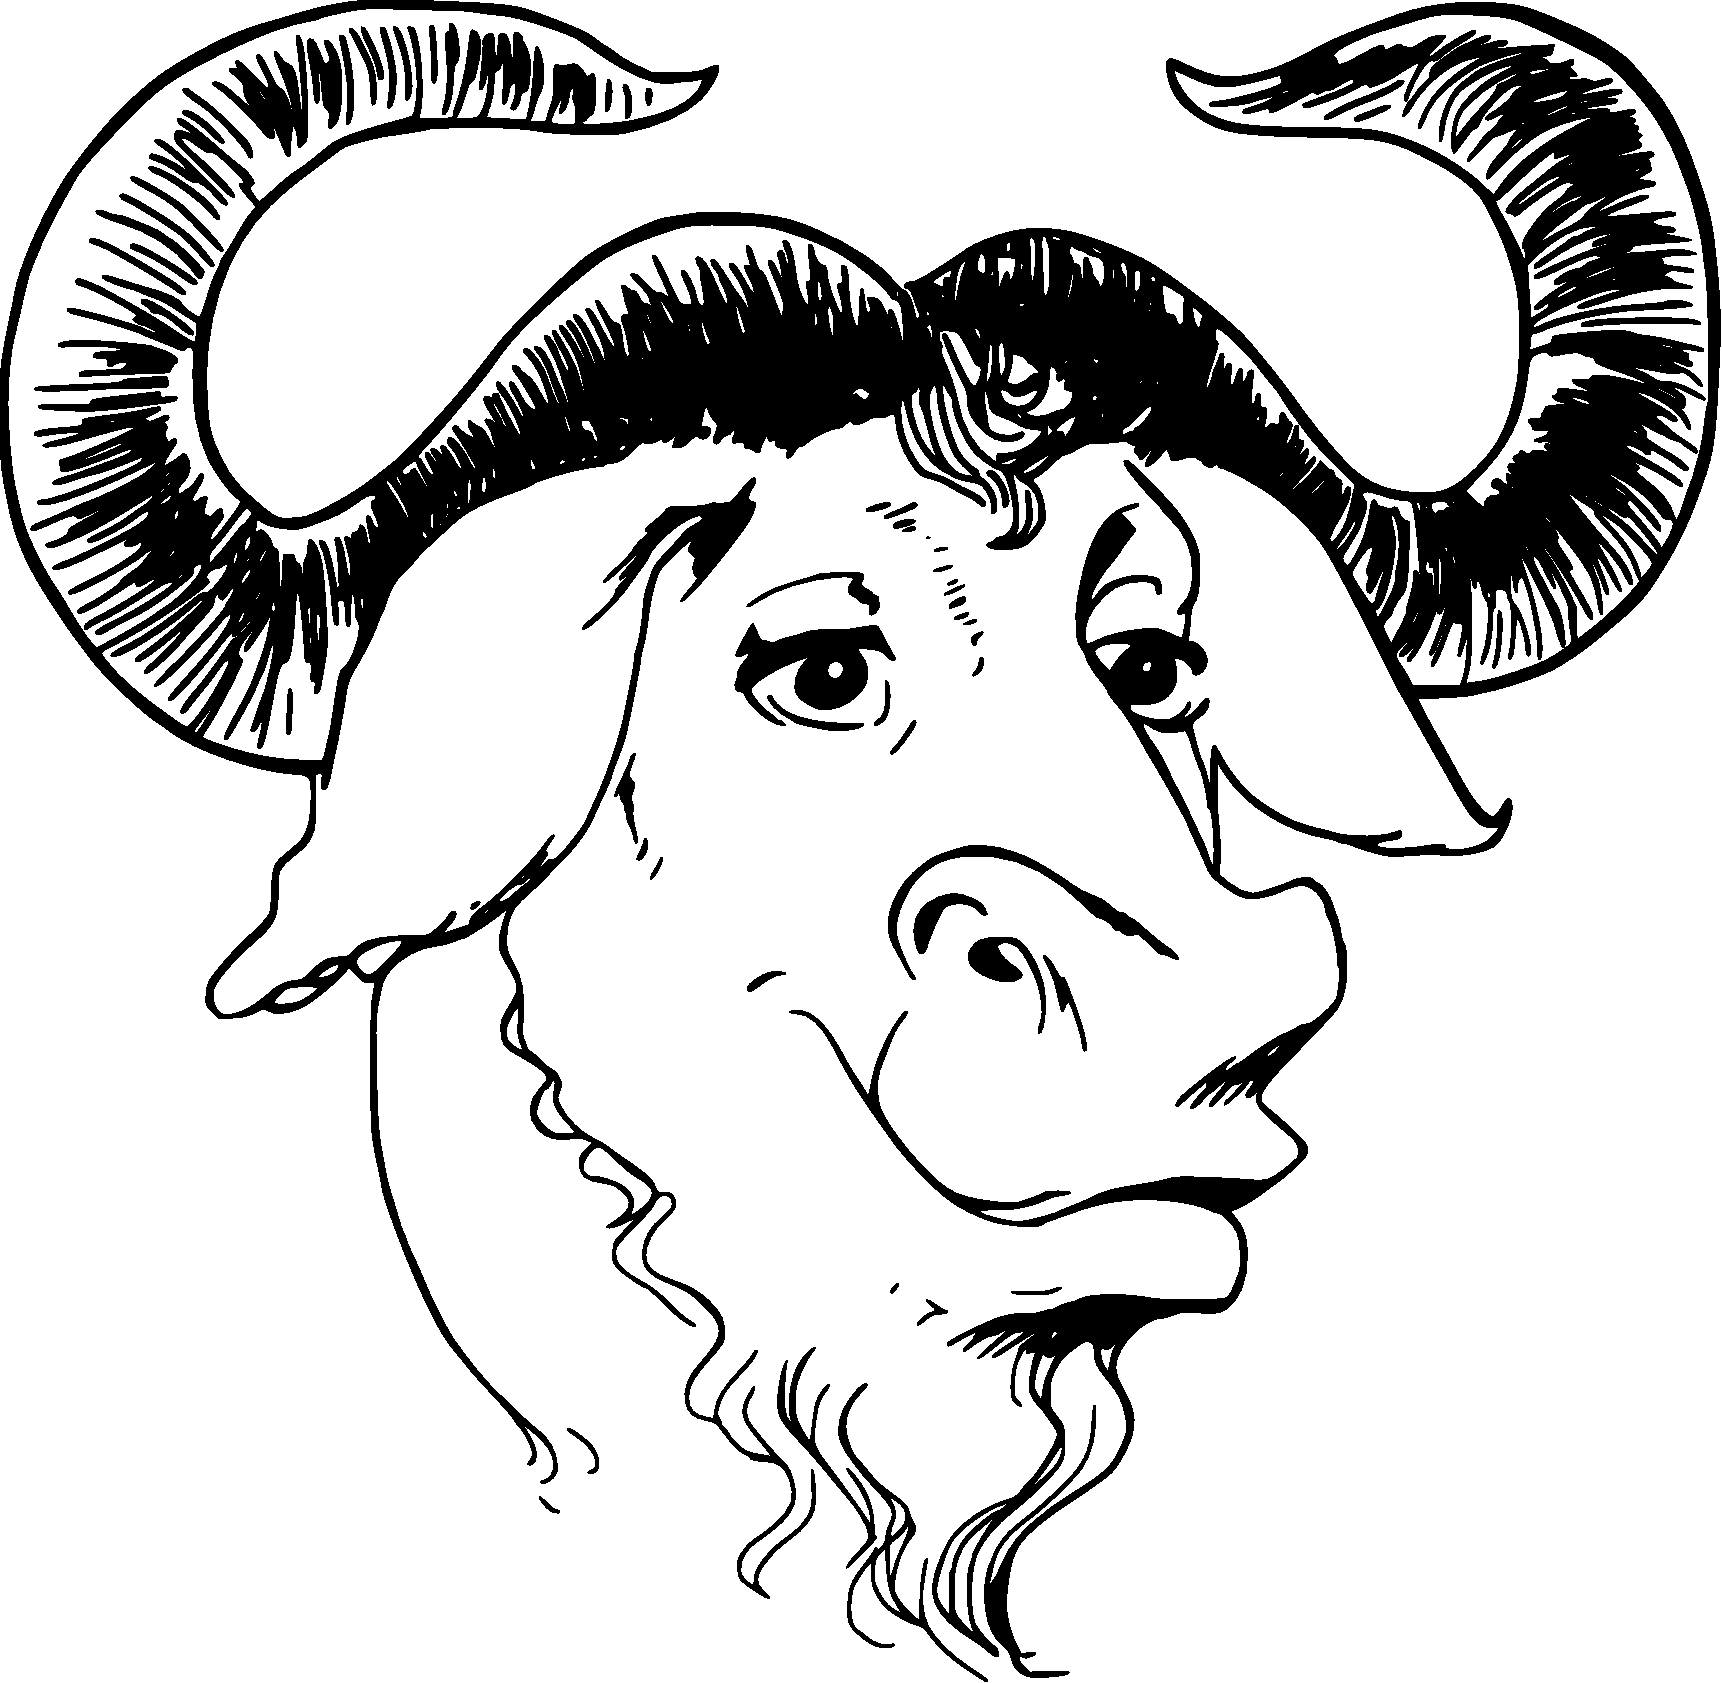
\includegraphics[width=\marginparwidth]{gfx/gnuhead_inkscape.pdf}}Sama praca udostępniana jest na zasadach otwartej licencji \textsc{GNU GPL 3.0}.

\section{Oprogramowanie mikrokontrolera}
W pracy wykorzystany został układ \textsc{AVR Atmega8}, będący ośmiobitowym mikrokontrolerem. Sprzęt ten znacznie różni się od architektury znanej z komputerów osobistych \textsmaller{PC} i choć sama idea programowania jest podobna, wszystko pozostawione jest programiście, co w połączeniu z koniecznością programowania na bardzo niskim poziomie, jaki nie jest promowany na studiach, stanowi dodatkowe wyzwanie.

Oprogramowanie zostało stworzone w języku \texttt{C}, wykorzystując do kompilacji kompilator \textsc{avr-gcc} oraz bibliotekę \textsc{avr-libc}, oba udostępniane na zasadach wolnej licencji \textsc{Modified Berkley License}. Do programowania wykorzystałem program \textsc{avrdude} (wolna licencja \textsc{GNU GPL 2} i późniejsze).

\subsection{Wymagania}
Zadaniem tej części oprogramowania jest dostarczenie danych, których obróbką zajmie się komputer. Wymagania, jakie są stawiane to przede wszystkim:
\begin{itemize}
 \item zwięzłość \ppauza program ma robić tylko i wyłącznie to, co absolutnie konieczne, ponieważ wprowadzanie dodatkowego, nadmiarowego kodu będzie powodowało opóźnienia w działaniu, co może przekładać się na
    niestabilność działania,
 \item dokładność \ppauza dostarczanie niepewnych danych mija się z celem pracy, należy więc zadbać o to, aby dane były możliwie najdokładniejsze,
 \item prostota \ppauza ze względu na niewielkie możliwości mikrokontrolera \ppauza w porównaniu do komputerów \ppauza trzeba zoptymalizować wszelkie używane struktury i unikać wykonywania pracy, którą spokojnie może zająć się komputer.
\end{itemize}

Uważam, że program, który napisałem spełnia wszystkie stawiane mu wymagania. Mieści się w niecałych 200 liniach \ppauza nie ma zbędnego kodu, dba o poprawne inicjalizowanie \index{timer}timerów urządzenia \ppauza stara się o dokładność danych, posiada możliwie najmniejsze struktury, które pozwolą przechować dane.

Należy zauważyć, że obrany rozmiar zmiennych, t.j. 8 bitów, został dopasowany do rozmiaru rejestrów mikrokontrolera. W przypadku zmiennych o długości 16 bitów znacznie wzrasta ilość taktów zegara, podczas których dane te są przetwarzane. Krótkie zmienne pozwalają na przechwycenie danych timera \ppauza rejestru \texttt{TCNT0} oraz licznika przepełnień \texttt{ovfCounter}\graffito{Rejestr \texttt{TCNT0} przechowuje aktualny stan licznika, a zmienna \texttt{ovfCounter} ilość cykli timera.} \ppauza w jednym takcie zegara.

Mikrokontroler posiada również drugi, szesnastobitowy timer, którego użycie pozwoliłoby na zwiększenie dokładności, wiązałoby się jednak z mankamentem wspomnianym powyżej, zaś precyzja osiągana przez oprogramowanie wykorzystujące timer o wielkości ośmiu bitów, jaka została opisana w sekcji \ref{section:microcontroller_limit}, jest wystarczająca do bardzo dokładnego śledzenia pozycji.

\subsection{Dokładność}\label{section:precision}
\paragraph{Ograniczenia mikrokontrolera}
\label{section:microcontroller_limit}

Dokładność, jaką można uzyskać za pomocą ośmiobitowego timera pracującego w układzie taktowanym zegarem $F_{cpu} = 8$ MHz wyznacza się w następujący sposób:
\begin{enumerate}
 \item \index{prescaler}prescaler\graffito{Prescaler omówiony zostanie w paragrafie \nameref{sec:prescaler} sekcji \ref{sec:uc_algorithm}} ustawiony jest na $F_{cpu}/8$, należy poznać interwał $i$, co jaki wyzwalane będzie przerwanie timera:
    \begin{equation}
      i = \frac{1}{F_{cpu}/8} = \frac{1}{1~\textrm{MHz}} = 0,000001~\textrm{s} = 0,001~\textrm{ms} = 1~\mu\textrm{s}
      \label{eq:sampling_frequency}
    \end{equation}

 \item znając interwał $i$ oraz szybkość dźwięku w powietrzu $v$, wyznaczyć należy drogę, jaką przebędzie dźwięk w czasie $i$, wykorzystując w tym celu wzór~\ref{eq:sound_distance}:
    \begin{equation}
      x = v \cdot i = 340~\frac{\textrm{m}}{\textrm{s}} \cdot 1~\mu\textrm{s} = 0,34~\textrm{mm}
      \label{eq:microcontroller_limit}
    \end{equation}
\end{enumerate}

Jak pokazuje równanie~\ref{eq:microcontroller_limit}\graffito{W praktyce należy uwzględnić jeszcze wymagania protokołu \ppauza patrz sekcja \ref{sec:protocol}}, teoretyczna dokładność sprzętu jest bardzo duża i znacznie przekracza wymagania gier wideo, gdzie w centrum zainteresowania są żwawe, gwałtowne ruchy. Pozwoliłaby ona na prawdopodobne wykorzystanie układu w zastosowaniach wymagających większej precyzji, jak np. modelowanie trójwymiarowe lub wizualizacja danych medycznych.

Ponieważ \index{timer}timer ma tylko osiem bitów, należy spodziewać się, że nastąpi jego przepełnienie zanim zostanie odczytane wygaszenie pinu. Przepełnienie wystąpi po dokładnie $2^8 = 256$ aktualizacjach timera. Zajmie to $256 \cdot 1~\mu\textrm{s} = 256~\mu\textrm{s}$, a dźwięk w tym czasie zdąży przebyć odległość 
\begin{equation}
 340~\frac{\textrm{m}}{\textrm{s}} \cdot 256~\mu\textrm{s} = 87,04~\textrm{mm}
\end{equation}

Rozdzielczość\graffito{Zmiana ta musiałaby zostać odwzorowana w aplikacjach wykorzystujących ten interfejs sterowania komputerem} można dalej zwiększyć zmniejszając dzielnik \index{prescaler}prescalera oraz zwiększając częstotliwość pracy mikrokontrolera.

\paragraph{Ograniczenia markerów}
\label{section:sound_limit}

Ze względu na wykorzystanie nadajników i odbiorników ultradźwiękowych używających dźwięku o częstotliwości $F_{d} = 40$ kHz, należy zbadać jakie narzuca to ograniczenia.

Podobnie jak w przypadku wyliczania ograniczeń mikrokontrolera, tak i w tym przypadku należy wyznaczyć minimalny interwał, w jakim może zajść zmiana.

Za zmianę będziemy przyjmować wygaszenie pinu mikrokontrolera, co spowodowane jest zaniknięciem nadawanego sygnału. Zdarzenie takie może zajść jedynie co pełny okres fali dźwiękowej. Policzmy więc odległość, jaka będzie dzieliła obraną fazę fali w dwóch ,,sąsiadujących'' okresach:

\begin{enumerate}
 \item wyliczamy okres $T$ fali dźwiękowej:
    \begin{equation}
      T = \frac{1}{F_d} = \frac{1}{40~\textrm{kHz}} = 0,000025~\textrm{s} = 0,025~\textrm{ms} = 25~\mu\textrm{s}
    \end{equation}
 \item znając $T$ skorzystajmy ponownie ze wzoru~\ref{eq:sound_distance}:
    \begin{equation}
      x = v \cdot T = 340~\frac{\textrm{m}}{\textrm{s}} \cdot 25~\mu\textrm{s} = 8,5~\textrm{mm}
      \label{eq:sound_limit}
    \end{equation}
\end{enumerate}

\paragraph{Teoretyczne ograniczenia całego systemu}
Jak pokazują obliczenia przeprowadzone w paragrafach~\nameref{section:microcontroller_limit} i~\nameref{section:sound_limit}, głównym ograniczeniem dokładności bieżącej wersji systemu jest wykorzystanie ,,powolnych'' nadajników i odbiorników.

Zdecydowałem się na wykorzystanie elementów \graffito{Należy spodziewać się, że czujniki stosowane np. w aparturze USG są odpowiednio drogie, wykorzystują jednak znacznie wyższe częstotliwości} o takich właśnie charakterystykach, ponieważ są to jedyne dostępne na rynku, których cena pozwala na ukończenie projektu.

Aby zwiększyć dokładność urządzenia należałoby wymienić nadajniki i odbiorniki na podobne modele, korzystające z wyższych częstotliwości, a także wymienić kwarc generujący częstotliwość dla tych elementów. Bez konieczności przeprogramowywania mikrokontrolera można zastosować elementy używające częstotliwości do
\begin{equation}
 f = \frac{1}{i} = \frac{1}{1~\mu\textrm{s}} = 1~\textrm{MHz}
\end{equation}
gdyż jest to częstotliwość próbkowania określona wzorem \ref{eq:sampling_frequency}\graffito{dodać info o możliwości podkręcenia częstotliwości przez zmniejszenie delay-ów oraz wysyłanie tylko impulsu, zamiast ciągłego sygnału, ponadto używanie w otwrtych przestrzeniach}.

\subsection{Algorytm}
\label{sec:uc_algorithm}
Oprogramowanie zapisane w pamięci mikrokontrolera steruje markerami i odbiornikami w następujący sposób:\graffito{metoda wyznaczania }
\begin{enumerate}
 \item \index{prescaler}prescaler urządzenia jest resetowany,\label{enum:prescaler}
 \item uruchamiany jest wewnętrzny licznik urządzenia,
 \item wysyłany jest sygnał, który aktywuje jeden z dwóch markerów, powoduje to rozpoczęcie nadawania sygnału przez ten marker,
 \item następuje aktywne oczekiwanie na ,,wygaszenie''\graffito{opisać czym jest wygaszenie} pinów wszystkich odbiorników,\graffito{Czas wygaszenia każdego z pinów (różnica czasu pomiędzy rozpoczęciem nadawania i odebrania sygnału z danego odbiornika) jest zapamiętywany}
 \item zatrzymywany jest wewnętrzny timer urządzenia,
 \item dane o odstępach czasowych przekazywane są do komputera,
 \item następuje uśpienie układu, które pozwala na zaniknięcie sygnałów ultradźwiękowych,
 \item cała operacja powtarzana jest dla drugiego markera.
\end{enumerate}
Algorytm ten obrazuje diagram przedstawiony na rysunku \ref{fig:firmware_sequence_diagram}.

\begin{figure}
 % fugly hack
 \hspace{-10em}
 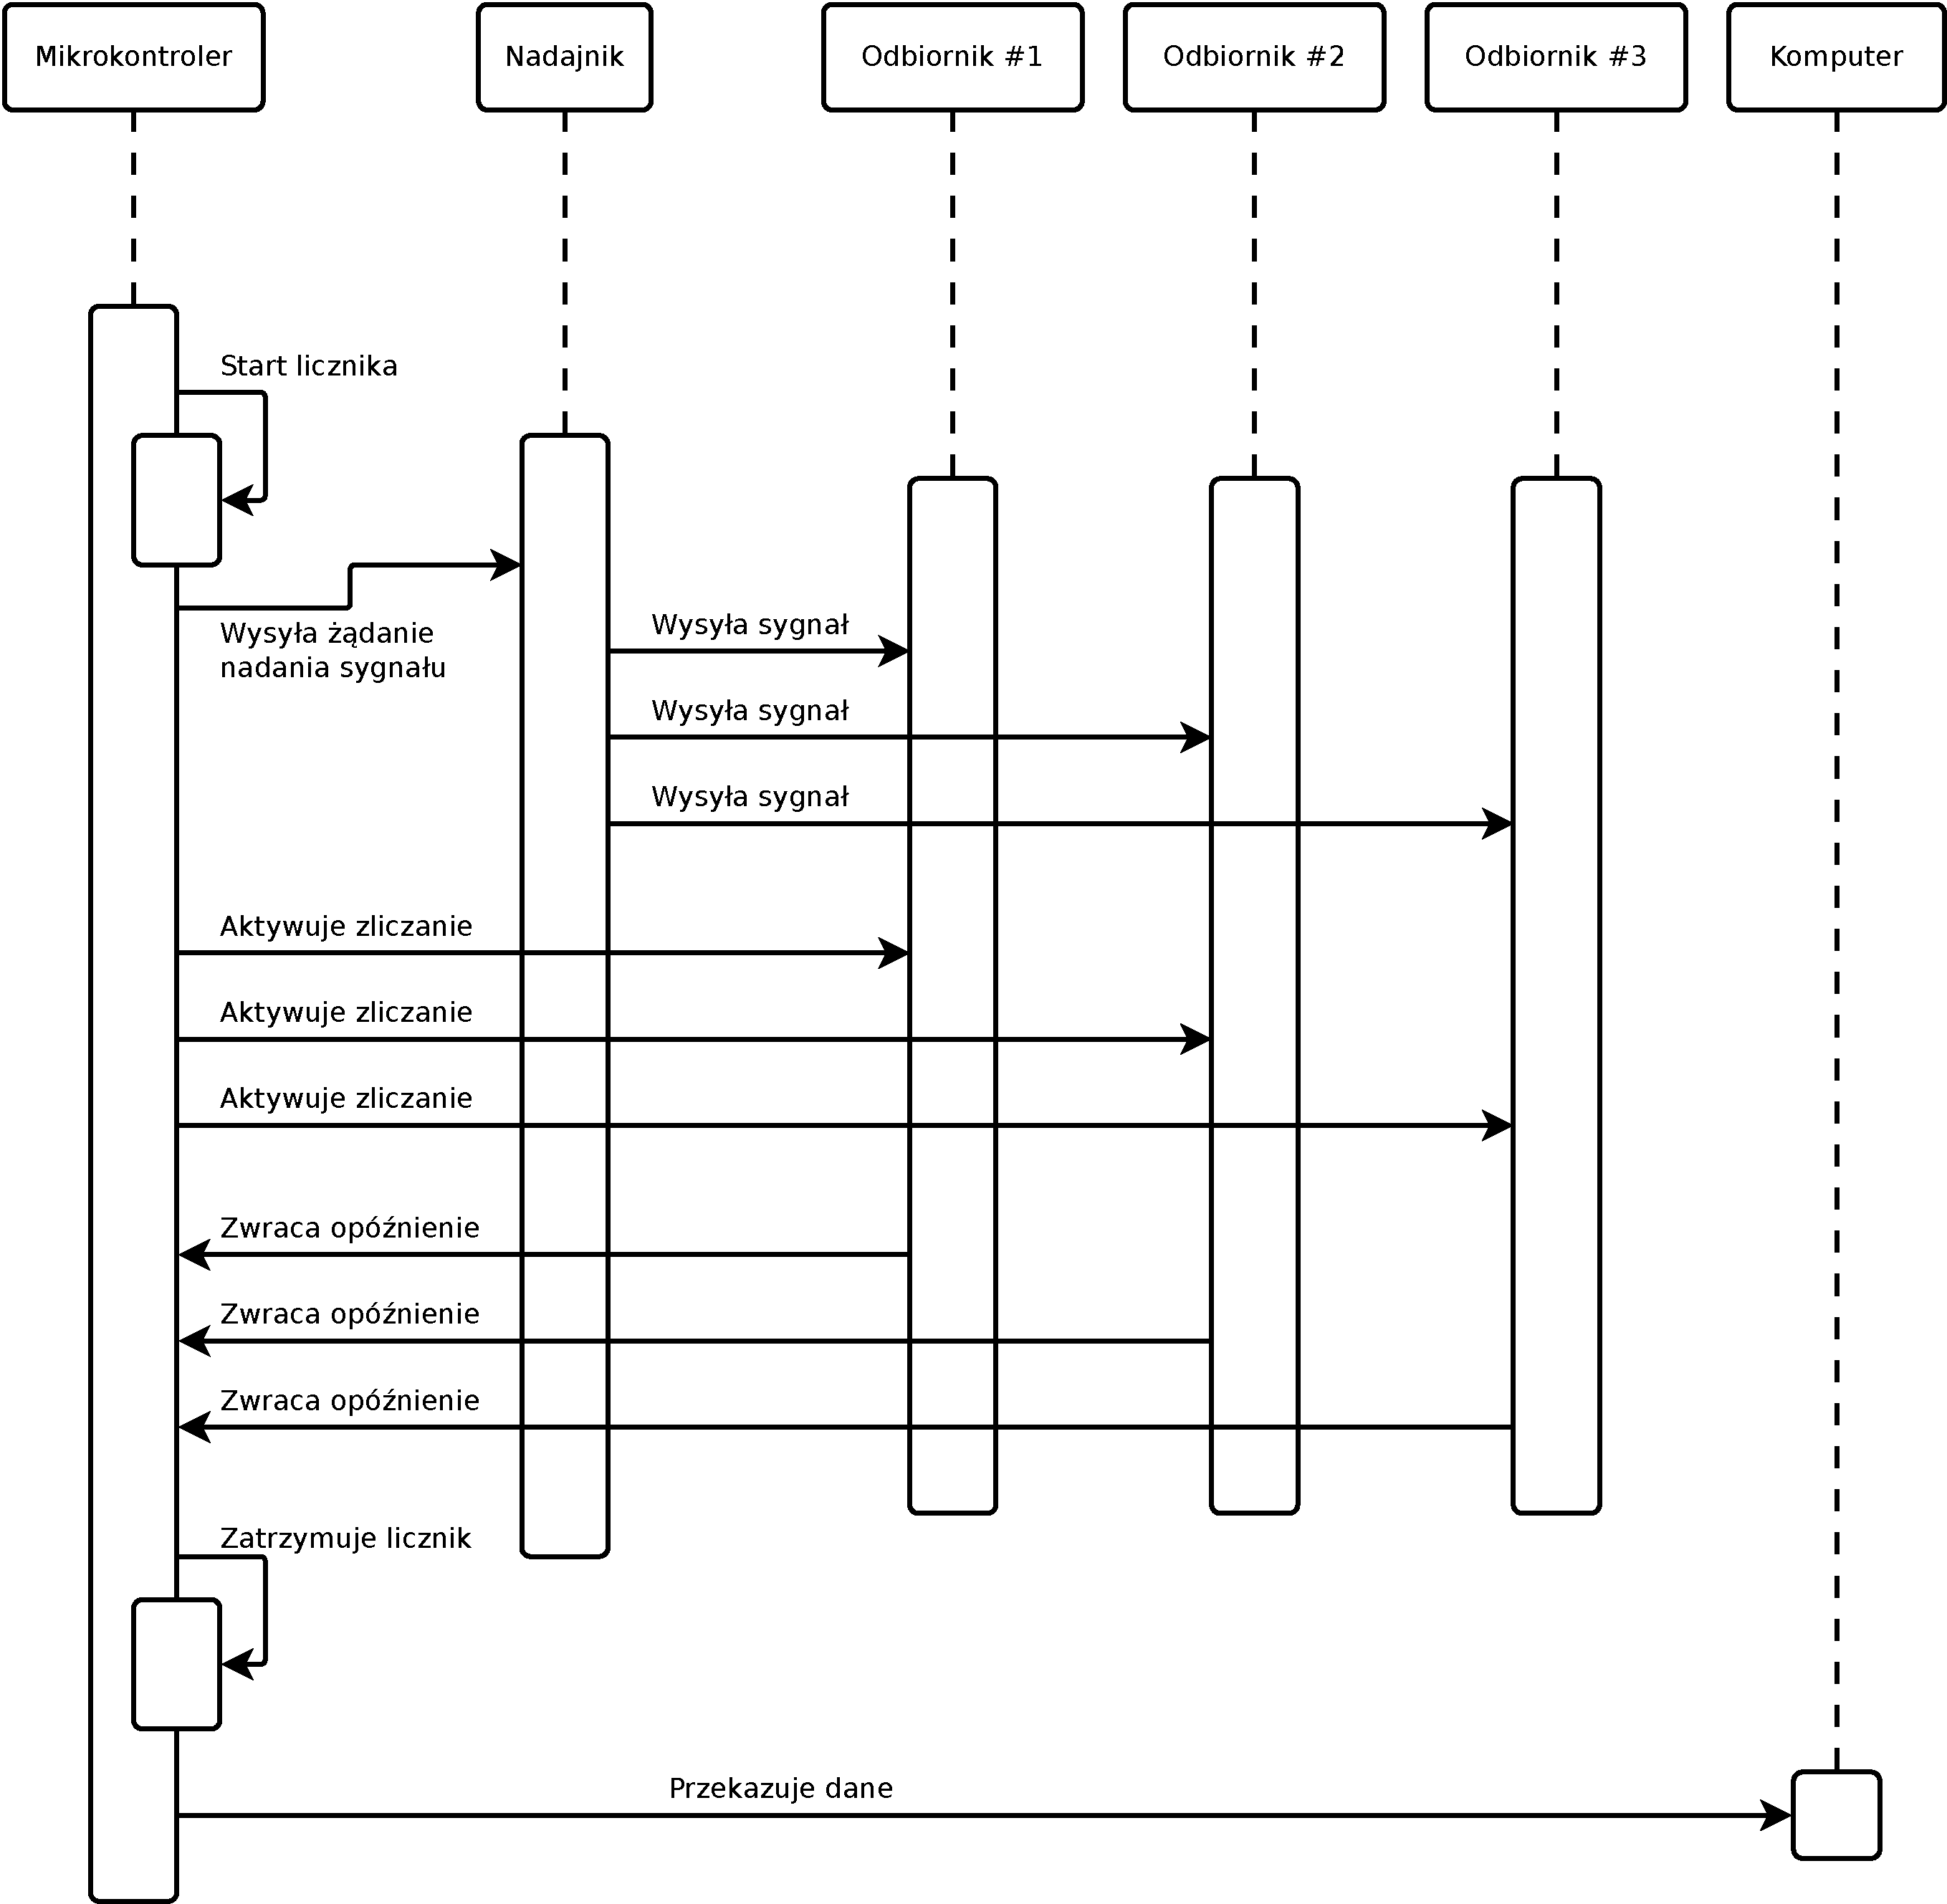
\includegraphics[width=45em]{gfx/diagramy/diagram_sekwencji_sprzetu.pdf}
 \caption{Diagram sekwencji oprogramowania mikrokontrolera}
 \label{fig:firmware_sequence_diagram}
\end{figure}

\paragraph{Prescaler}
\label{sec:prescaler}
W mikrokontroler wbudowany jest \index{prescaler}\textsl{prescaler}, czyli dzielnik częstotliwości, o programowanym stopniu podziału. Jego działanie polega na zliczaniu taktów zegara; gdy wewnętrzny licznik prescalera osiągnie zaprogramowaną wcześniej wartość, wyzwalane jest przerwanie timera oraz następuje przepełnienie licznika, w związku z czym zliczana wartość ,,przekręca się'' i liczenie rozpoczyna się ponownie od zera.

Punkt \ref{enum:prescaler} algorytmu jest bardzo istotny, gdyż nie ma możliwości\graffito{Nawet gdyby możliwość odczytania tej wartości istniała, działanie to wprowadzałoby niepożądane opóźnienia} sprawdzenia aktualnego stanu licznika prescalera, natomiast rozpoczęcie odliczania może nastąpić w dowolnym momencie czasu, przez co może być niekoniecznie zsynchronizowane z wyzwoleniem przerwania przez prescaler, efektem czego byłyby pomiary, które charakteryzowałyby się pewną zmienną niedokładnością.

\paragraph{Przerwania}
W działaniu programu dużą rolę odgrywają procedury obsługi przerwań (ang. \textsl{ISR \ppauza Interrupt Service Routine}). Są to krótkie fragmenty kodu, które wywoływane są przez mikrokontroler w przypadku zajścia pewnego zdarzenia. Ich użycie pozwala na pewien stopień ,,wielowątkowości'', gdyż (w zależności od ustawienia flag) mogą one przerwać wykonywanie głównego toku programu do momentu, aż przerwania nie zostaną ,,obsłużone'', tzn. instrukcje zawarte w procedurze ISR nie zostaną wykonane.

Implementacja procedur obsługi przerwań jest rozszerzeniem języka C, która jest charakterystyczna dla wybranej rodziny układów i wykorzystanego kompilatora, co powoduje, że wykorzystanie innego kompilatora lub innej rodziny układów wymaga przepisania procedur ISR zgodnie z nowymi wymaganiami.

Jednym z wykorzystanych przerwań jest przerwanie wywoływane przez moduł \texttt{Timer/Counter0}: \texttt{Timer/Counter0 Overflow} (\texttt{TOV0}). Jest ono wyzwalane, gdy licznik \texttt{TCNT0} przekroczy maksymalną możliwą dla niego wartość i rozpocznie się ponowne odliczanie od zera. Zadaniem zawartego w tej procedurze kodu jest tylko i wyłącznie inkrementacja zmiennej \texttt{ovfCounter}, dzięki czemu znana jest ilość przepełnień licznika. W przypadku pominięcia tej danej, pomiary ograniczony byłyby do zaledwie 256 możliwości odległości markera od odbiornika.

Drugie wykorzystane przerwanie jest również przerwaniem licznika i wyzwalane jest przez moduł \texttt{Timer/Counter1}. Jedynym zadaniem tego przerwania jest obsługa jednej z diod, której zadaniem jest wizualne potwierdzenie sprawności i działania układu.

Przykład procedury obsługi przerwania na podstawie opisanej właśnie funkcjonalności prezentuje listing~\ref{lst:interrupt_handler}.

\begin{listing}
  \lstinputlisting[language=C]{listings/atmega_interrupt.c}
  \caption{Procedura obsługi przerwania \texttt{Timer/Counter0 Overflow}}
  \label{lst:interrupt_handler}
\end{listing}

Oznaczenie zmiennej jako \texttt{volatile} oznajmia kompilatorowi, że wszelkie odczyty i zapisy muszą operować na wartości zmiennej z pamięci. W przypadku braku takiego zapisu kompilator podczas kompilowania kodu źródłowego z włączoną flagą optymalizacji może przyjąć, że procedura zmieniająca wartość zmiennej nie jest nigdzie wywoływana, przez co bezpiecznym jest cache-owanie wartości zmiennej, a w efekcie zignoruje skutki wywołania przerwania.

Makro \texttt{ISR(vector [, attributes])} z biblioteki \textsmaller{avr-libc} definiuje następujące po nim ciało funkcji jako procedurę obsługi przerwania. Argument \texttt{vector} jest wymagany i oznacza pozycję w wektorze przerwań mikrokontrolera, do której przypisany ma zostać kod. Argument \texttt{attributes} jest opcjonalny i modyfikuje działanie procedury ISR \ppauza pozwala np. na zagnieżdżanie przerwań, czyli przerwanie przetwarzania procedury ISR przez inne przerwanie.

Wygenerowany wektor przerwań, prezentujący obecność tylko dwóch, wymienionych powyżej, procedur obsługi przerwania prezentuje listing~\ref{lst:interrupt_vector}.

\begin{listing}
  \lstinputlisting{listings/interrupt_vector.txt}
  \caption[Wektor obsługi przerwań]{Wygenerowany wektor obsługi przerwań}
  \label{lst:interrupt_vector}
\end{listing}

Pierwsza pozycja na liście jest punktem wejścia programu, od którego rozpoczyna się wykonywanie kodu. Pozycje z adresów \texttt{0x10} i \texttt{0x12} to przekierowania do odpowiednio procedur ISR dla przerwań \texttt{Timer/Counter0 Overflow} i \texttt{Timer/Counter1 Overflow}.

\section{Oprogramowanie dla komputera}
W celu stworzenia oprogramowania dla komputera wykorzystałem kilka środowisk i bibliotek.

\paragraph{Qt}
Wieloplatformowe środowisko (ang. \textsl{framework}) \textsmaller{Qt}, licencjonowane wolną licencją \textsc{GNU LGPL 2.1} oraz \textsc{GNU GPL 3.0}, składa się z kilku komponentów. W jego skład wchodzą między innymi: biblioteka \textsc{Qt} oraz kompilator \verb|moc|. Wszystkie te elementy znacznie usprawniają pisanie aplikacji w języku \verb|C++| dostarczając metod, które abstrahują od specyfiki wykorzystywanego systemu operacyjnego.

Pisanie nawet skomplikowanych programów z wykorzystaniem \textsc{Qt} jest proste, łatwe, szybkie i przyjemne. Programista świadomy różnic pomiędzy systemami operacyjnymi i delegujący obsługę parametrów do metod dostarczanych przez klasy bibliotek \textsc{Qt} zyskuje możliwość skompilowania swojego kodu pod platformy \textsc{Linux}, \textsc{Windows} oraz \textsc{Mac OS X} bez konieczności jakichkolwiek zmian.

Szerokie spektrum dostarczanych klas (począwszy od kontenerów danych i metod iteracji, przez obsługę urządzeń wejściowych, przez obsługę sieci, aż po rysowanie i zarządzanie grafikami i wiele, wiele innych\ldots) zapewnia, że do zaimplementowania wielu aplikacji nie będzie wymagane wykorzystanie bibliotek trzecich.
\newline
\newline
\textsl{Sygnały i sloty}
Ze względu na intensywne wykorzystywanie w stworzonych aplikacjach połączeń sygnał-slot, zamieszczam poniżej ich opis.

Centralną właściwością środowiska \textsc{Qt}, a jednocześnie jedną z najbardziej odróżniających ten framework od innych, jest mechanizm sygnałów i slotów będący zarządzaną metodą komunikacji pomiędzy obiektami.

Chociaż na pierwszy rzut oka przypomina ona znane dotychczas metody oparte o wywołania zwrotne (ang. \textsl{callback}) i faktycznie się z nich wywodzi, to jednak różni się od nich w kilku kluczowych aspektach.

Jest to metoda dynamiczna (działająca w runtime). Metoda wywołań zwrotnych wykorzystywana jest głównie do zamodelowania statycznych (tj. znanych już podczas czasu kompilacji - ang. \textsl{compiletime}) powiązań pomiędzy obiektami jak np:
\begin{verse}
użytkownik kliknął przycisk \texttimes~\textrightarrow~wywołaj metodę \texttt{close()}
\end{verse}

W przypadku tym przypisuje się wskaźnik do funkcji do pewnego pola klasy wywołującej, który w momencie zajścia zdarzenia jest wywoływany. Konsekwencją takiego podejścia jest konieczność znania odbiorników w czasie kompilacji, co uniemożliwia np. ładowanie wtyczek w runtime i powiadamiania ich o zdarzeniach w następujący sposób:
\begin{verse}
powiadom wszystkie odbiorniki o zajściu zdarzenia $\omega$
\end{verse}

Zastosowanie w tym miejscu wektorów wskaźników jest jedynie obejściem problemu, a nie jego rozwiązaniem, gdyż nakłada na programistę obowiązek pamiętania o poprawnym przydzielaniu i zwalnianiu pamięci na te elementy, w przypadku aplikacji wielowątkowych szczegółowego analizowania zależności czasowych pomiędzy wywołaniami kodu obiektów, oraz drobiazgowego sprawdzania typów wywołań.

Podejście to wprowadza ponadto nadmiarową i zbędną wiedzę o odbiornikach do nadajnika.

Rozwiązanie dostarczane przez framework \textsc{Qt} jest elegancką metodą pozbycia się wymienionych wad na rzecz udostępnienia programiście prostego w obsłudze, lecz potężnego i skutecznego, mechanizmu dynamicznego wiązania obiektów w pary nadajnik-odbiornik.

Przekazywane sygnały są ,,wątkowo-bezpieczne'' (ang. \textsl{thread-safe}), co pozwala na przetwarzanie sygnału w innym wątku niż ten, który zainicjował jego wysłanie. Aby zrealizować takie podejście, każdy z obiektów dziedziczących po klasie \verb|QObject| powinien należeć do jakiegoś wątku, tak aby był on uwzględniany w pętli zdarzeń (ang. \textsl{event loop}), jaka jest przez ten wątek przetwarzana. Domyślnie każdy nowy obiekt przynależy do wątku rodzica, który go utworzył.

Pociąga to za sobą konsekwencję, że jeżeli obiekt nie przynależy do żadnego wątku, to jego zdarzenia nie będą przetwarzane.

W celu uproszczenia obsługi, środowisko \textsc{Qt} domyślnie wykorzystuje do wszystkich obiektów wątek główny aplikacji i jeśli programista jawnie nie usunie z niego obiektów, to ich sygnały będą przetwarzane właśnie w tym wątku.

Aby zintegrować to rozwiązanie z kodem, postanowiono ,,rozszerzyć'' standard\graffito{,,Rozszerzenie'' to wykorzystywane jest tylko i wyłącznie do środowiskia \textsc{Qt}} języka \verb|C++|. Do istniejących już kwalifikatorów \verb|public|, \verb|private| i \verb|protected| dodano dwa nowe: \verb|signals| i \verb|slots|.

Kwalifikator \verb|signals| definiuje sygnały. Mają one taką samą strukturę, jak zwykłe metody klasy z następującymi wyjątkami:
\begin{aenumerate}
  \item definicja sygnału jest tylko i wyłącznie jego deklaracją, oznacza to, że sygnał nie posiada żadnego kodu, jest tylko abstrakcyjnym tworem komunikującem zajście pewnego zdarzenia,
  \item sygnały nie mogą zwracać wartości \ppauza zwracanym typem musi być \verb|void|, a wszelkie przekazywane dane zawarte są w argumentach,
  \item sygnały są zawsze publiczne.
\end{aenumerate}

Deklarację pewnej minimalnej klasy zawierającej sygnały prezentuje listing \ref{lst:signals_declaration}.

\begin{listing}
  \lstinputlisting{listings/signals_declaration.cpp}
  \caption{Klasa zawierająca sygnały}
  \label{lst:signals_declaration}
\end{listing}

Jak pokazano, aby klasa mogła wykorzystać mechanizm sygnałów (a także slotów), musi ona dziedziczyć z klasy \verb|QObject| i wywoływać makro \verb|Q_OBJECT| w prywatnej części deklaracji.

Kwalifikator \verb|slots|, jak łatwo się domyślić, deklaruje sloty. Poza dodatkową możliwością wywołania slotu, są to tradycyjne metody klasy i tak samo obowiązują je pozostałe kwalifikatory: \verb|public|, \verb|private| i \verb|protected|. W odróżnieniu od sygnałów, sloty wymagają dostarczenia implementacji i mogą zwracać wartości.

Deklarację pewnej minimalnej klasy zawierającej sloty prezentuje listing \ref{lst:slots_declaration}.

\begin{listing}
  \lstinputlisting{listings/slots_declaration.cpp}
  \caption{Klasa zawierająca sloty}
  \label{lst:slots_declaration}
\end{listing}

Połączenie emitera ze słuchaczem następuje poprzez wywołanie metody \verb|connect| klasy \verb|QObject|, której argumentami są obiekty nadający i odbierający, a także nazwy łączonych metod. Sygnatura slotu i sygnału musi być taka sama, z wyjątkiem zwracanego typu.

Użyteczną cechą jest możliwość podłączenia sygnału do sygnału, dzięki czemu zostanie wywołany drugi z sygnałów, a w efekcie podłączone do niego sloty.

Pozostała charakterystyka tego rozwiązania, taka jak przekazywanie meta-typów, rozgraniczenie pomiędzy obiektem nadającym, a odbierającym oraz inne, nie została wykorzystana w stworzonym oprogramowaniu, w związku z czym odsyłam czytelnika do dokumentacji środowiska \textsc{Qt} \citep{Qt}.
\newline
\newline
\textsl{Kompilator moc} Ponieważ powyższe rozwiązanie nie należy do standardu języka \verb|C++|, zaś całe oprogramowanie stworzone przy pomocy środowiska \textsc{Qt} kompilowane jest przy pomocy kompilatora \verb|C++| zgodnego ze standardem ANSI C++\graffito{jaki to dokłądnie standard i skąd?}, takiego jak \texttt{g++}, dostarczany jest wraz z \textsc{Qt} kompilator \texttt{moc}, czyli \textsl{meta-object compiler}.

Zadaniem tego narzędzia jest przeparsowanie dostarczonych plików źródłowych pod kątem odszukania wśród nich deklaracji klas dziedziczących z \verb|QObject|, a zatem wykorzystujących rozszerzone możliwości oferowane przez \textsc{Qt} i wygenerowanie kodu zrozumiałego przez wspomniany wyżej ,,zwykły'' kompilator. Kod dostarczony przez programistę, pozbawiony rozszerzeń \textsc{Qt} oraz kod wygenerowany przez narzędzie \texttt{moc} są kompilowane, a następnie łączone ze sobą na etapie linkowania.

\paragraph{QSerialPort}
Biblioteka \textsc{QSerialPort}, oparta o wolną licencję \textsc{GNU LGPL 2.1}, dostarcza metod komunikacji wykorzystujych port szeregowoy \textsmaller{RS232}. Opiera się ona o środowisko \textsc{Qt}, przez co bardzo łatwo jest zintegrować ją z projektami korzystającymi z tych narzędzi. Podobnie jak samo \textsc{Qt}, biblioteka ta jest wieloplatformowa, co było jednym z głównych powodów, dla których wybrałem właśnie ją.

Dostarcza ona metody obsługi portów oparte o interfejs \verb|QIODevice| udostępniany przez \textsc{Qt}, które implementowane są z wykorzystaniem natywnych funkcji systemowych dla każdej z platform, dzięki czemu przekazywanie danych odbywa się szybko i sprawnie.

\paragraph{Qwt}
Zadaniem tej biblioteki\graffito{\textsc{QWT} oznacza \textsc{Qt Widgets for Technical Applications}}, opartej o wolną licencję \textsc{Qwt License 1.0} (która z kolei oparta jest o licencję \textsc{GNU LGPL 2.1}), jest rysowanie i obsługa wykresów. Jest ona, podobnie jak \textsc{QSerialPort}, oparta o środowisko \textsc{Qt}, co zapewnia niedostępny w innym przypadku poziom integracji. Ponieważ poza \textsc{Qt} oraz standardową biblioteką \textsc{libstdc++} nie posiada ona żadnych zewnętrznych zależności, to podobnie jak te projekty jest ona także wieloplatformowa.

\paragraph{Bazaar}
\textsc{Bazaar} lub, w skrócie, \textsc{bzr}\graffito{Skrót wziął się od nazwy wykonywanego polecenia \ppauza \texttt{bzr}}, to dystrybuowany system kontroli wersji, który pozwala na śledzenie i oznaczanie zmian w kodzie źródłowym, dzięki czemu można śledzić rozwój programu, oznaczać wydania, współdzielić kod pomiędzy gałęziami,  przypisywać błędy do rewizji oraz wiele innych. W połączeniu z serwisem \textsc{Launchpad} umożliwia hostowanie kodu w repozytorium on-line oraz wygodne zarządzanie projektem. Oba narzędzia udostępniane są na zasadach wolnych licencji, odpowiednio: \textsc{GNU GPL 2} i późniejsze oraz \textsc{GNU Affero GPL v3}.

Całość stworzonej pracy, włączając w to ten dokument, wersjonowane były wykorzystując te narzędzia i należą do projektu \texttt{janisozaur-inz} dostępnego pod adresem:
\begin{verse}
  \url{https://launchpad.net/janisozaur-inz}
\end{verse}

\subsection{Trilaterator}
Pierwsza ze stworzonych aplikacji przeznaczona jest do przeprowadzania trilateracji, o której mowa w sekcji \ref{par:trilateration}. Wykonuje ona automatycznie obliczenia dane wzorami \ref{eq:trilateration_final_x}, \ref{eq:trilateration_final_y} i \ref{eq:trilateration_final_z}. Interfejs aplikacji umożliwia wprowadzanie wszelkich danych dotyczących rozmieszczenia odbiorników jak i markera. Wyniki dokonanych obliczeń prezentowane są w dolnej części programu.

Aplikację wraz z przykładowymi danymi prezentuje rysunek \ref{fig:trilaterator}.

\begin{figure}[t]
 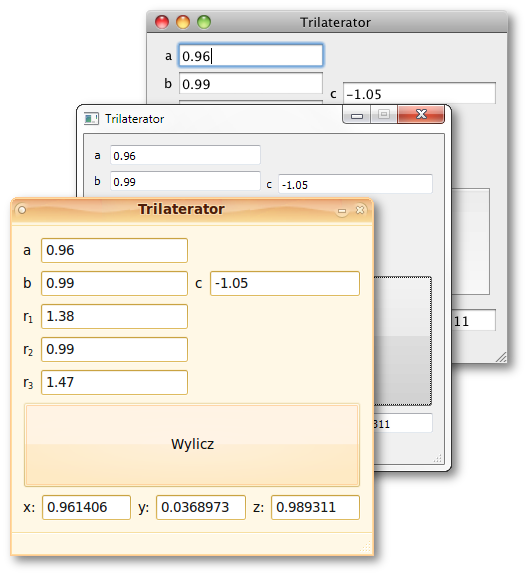
\includegraphics[width=\textwidth]{gfx/trilaterator_triple.png}
 \caption{Trilaterator. Aplikacja dokonująca trilateracji}
 \label{fig:trilaterator}
\end{figure}

Przykładowe dane oraz poprawność zastosowanej metody pokazuje rysunek \ref{fig:trilateration_sample}.

Jak widać, oddalenie odbiorników od siebie na odległość zaledwie kilku centymetrów pozwala badać położenie markera w przestrzeni.

\paragraph{Struktura programu}
Przedstawiony program jest celowo bardzo prosty i sprowadza się tylko do obsługi zdarzenia kliknięcia przycisku, tak aby łatwo można było prześledzić działanie metody. Całą istotę działania programu prezentuje listing~\ref{lst:trilateration}.

\begin{listing}
  \lstinputlisting{listings/trilateration.cpp}
  \caption{Kod dokonujący trilateracji}
  \label{lst:trilateration}
\end{listing}

\paragraph{Dokładność obliczeń}
Należy wziąć pod uwagę fakt, że odległość pomiędzy odbiornikami ma wpływ na wynik obliczeń. Wynika to z operowania przez komputer na danych o skończonej i zmiennej dokładności.

Jeśli marker znajdzie się dostatecznie daleko od odbiorników, może nastąpić spadek precyzji, gdyż dane są reprezentowane w pamięci komputera przez typy zmiennoprzecinkowe i przy małym rozsunięciu odbiorników po wykonaniu działań arytmetycznych, a w szczególności operacji potęgowania i pierwiastkowania, jakie są konieczne do odtworzenia pozycji, utrata precyzji będzie miała znaczący wpływ na wynik obliczeń.

Aby uniknąć tego problemu, odbiorniki \textsl{Nietoperza} rozstawione są na planie trójkąta równobocznego o boku 33cm. Pozwala to na wystarczająco dokładne śledzenie precyzji już za pomocą typu zmiennoprzecinkowego pojedynczej precyzji \verb|float|. Na potrzeby tej demonstracji zdecydowałem się jednak wykorzystać typ \verb|double| dostarczający podwójnej precyzji.

\paragraph{Wieloplatformowość}
Aplikacja ta prezentuje także zalety wykorzystanego środowiska, które może być kompilowane pod wszystkimi trzema znaczącymi systemami operacyjnymi: \textsl{Linux}, \textsl{Windows} i \textsl{Mac OS X}. Do poprawnego skompilowania nie jest wymagana żadna zmiana kodu.

\begin{figure}
  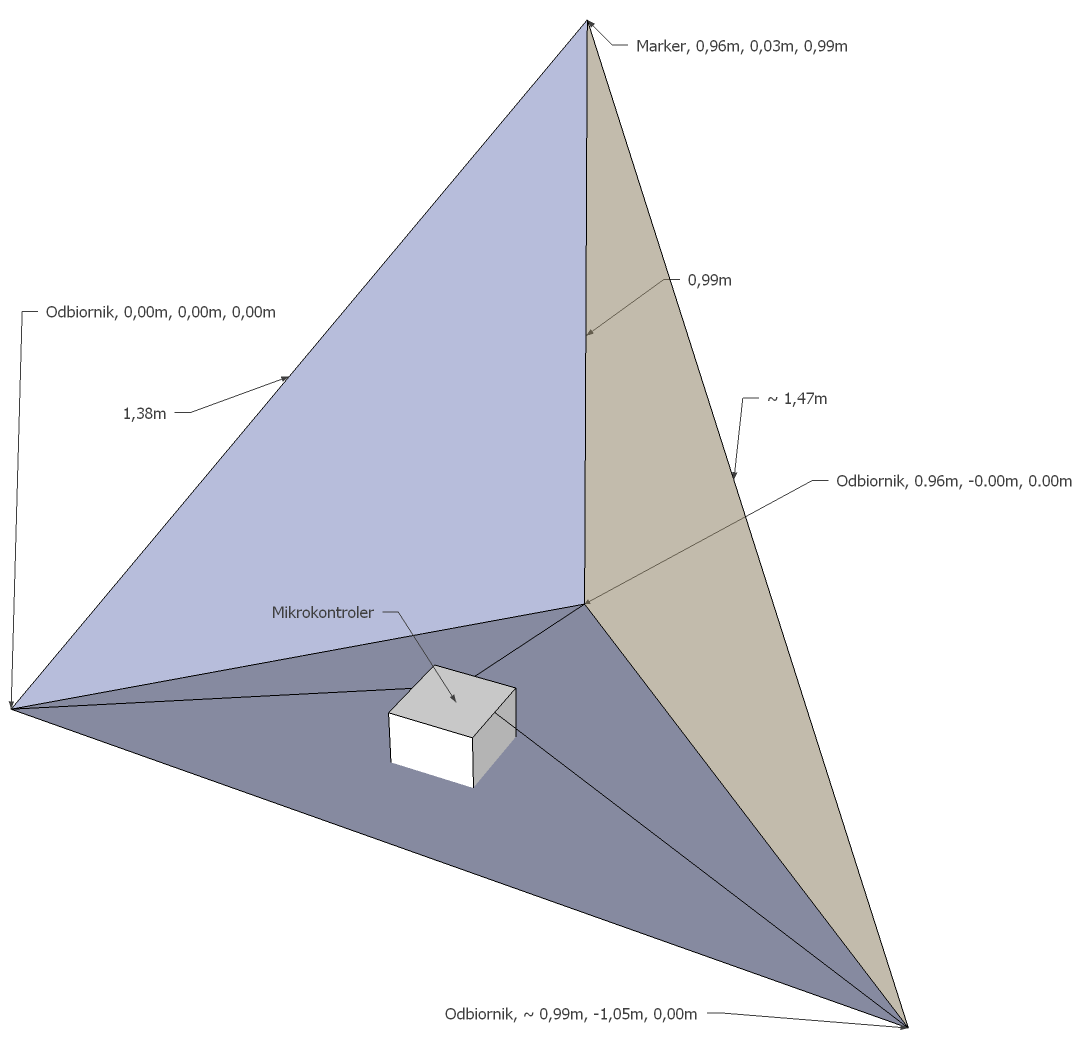
\includegraphics[width=\textwidth]{gfx/wizualizacja_3d.png}
  \caption{Wizualizacja przykładowych danych}
  \label{fig:trilateration_sample}
\end{figure}

\begin{figure}
 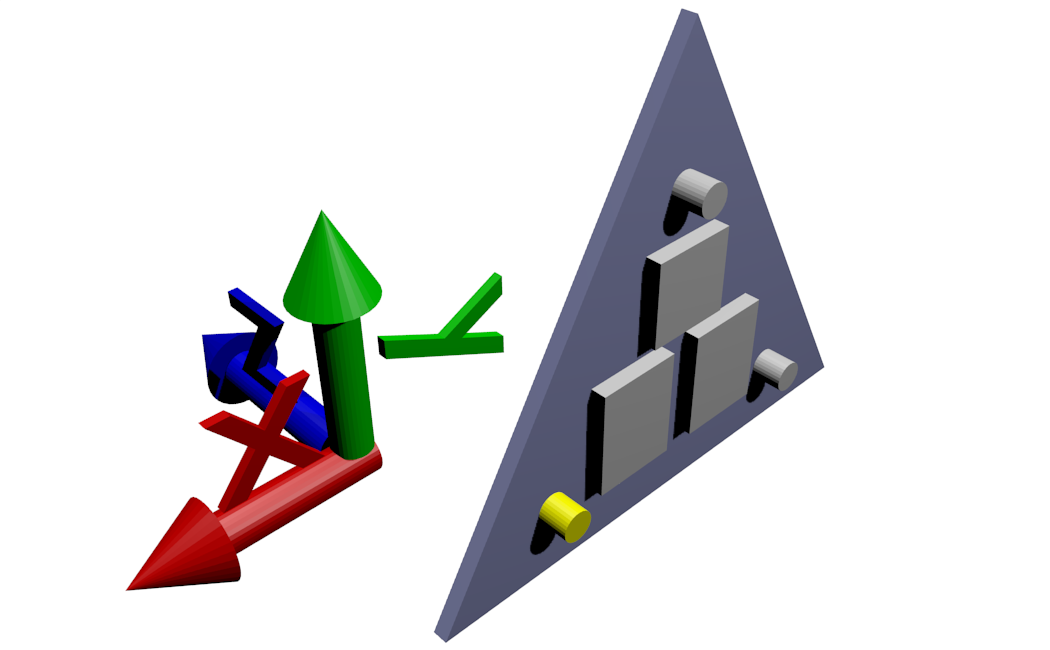
\includegraphics[width=\textwidth]{gfx/uklad_render.png}
 \caption[Model systemu i przyjęty układ współrzędnych]{Model systemu wraz z przyjętym układem współrzędnych. Układ ma swój początek w odbiorniku oznaczonym kolorem żółtym}
 \label{fig:coordinate_system}
\end{figure}

\subsection{Charter}
Kolejna aplikacja prezentująca możliwości systemu służy do rysowania wykresów w czasie rzeczywistym na podstawie danych pobranych z mikrokontrolera. Dla porównania dostępne są dwa rodzaje wykresów jednocześnie:
\begin{itemize}
 \item odległość od odbiornika \ppauza pokazuje odległość wybranego markera od każdego z odbiorników,
 \item położenie \ppauza dokonuje w locie trilateracji dla bieżącej próbki i rysuje wykres położenia wybranego markera w trzech wymiarach, zgodnie z układem odniesienia przedstawionym na rysunku \ref{fig:coordinate_system}.
\end{itemize}

Odległość od odbiorników podawana jest jako wartość licznika odczytana z mikrokontrolera. Aby dokonać konwersji na centymetry, należy (w oparciu o równanie \ref{eq:microcontroller_limit}) przeliczyć:
\begin{equation}
 d = \frac{x \cdot 0,34\textrm{mm}}{10}
\end{equation}
gdzie:
\begin{description}
 \item[$d$] \ppauza~wyznaczona odległość w centymetrach,
 \item[$x$] \ppauza~odległość odczytana z wykresu.
\end{description}

Użytkownik w trakcie działania programu ma możliwość wyboru, którego markera dane powinny być rysowane.

Program dokonuje transformacji układu współrzędnych, aby w efekcie uzyskać układ pokazany na rysunku \ref{fig:coordinate_system}.

Jest to taki sam prawoskrętny układ, jak wykorzystywany w bibliotece \textsc{OpenGL}, co znacząco ułatwia pracę, ponieważ nie jest wymagana żadna dodatkowa konwersja układu współrzędnych aby narysować pozycję markera.

\paragraph{Struktura programu}
Program napisany jest z wykorzystaniem środowiska \textsc{Qt}, ponadto korzysta z bibliotek \textsc{QSerialPort} oraz \textsc{Qwt}.

Po uruchomieniu programu tworzone są obiekty wykresów \verb|PositionPlot| i \verb|DistancePlot|, które dziedziczą z klasy \verb|QwtPlot| i zajmują się rysowaniem odpowiednio wykresów pozycji markera oraz jego odległości, ustawiane są parametry tych obiektów dotyczące skali, legendy oraz uruchamiane są timery odpowiadające za odświeżanie danych. Wykresy przedstawiają dane pobrane w ciągu ostatnich 10 sekund i wraz z przybywaniem kolejnych danych wykres jest przesuwany aby spełnić wymieniony właśnie warunek.

Następuje inicjalizacja pozostałych danych interfejsu użytkownika:
\begin{itemize}
  \item domyślny adres portu szeregowego \ppauza jest to jeden z dwóch fragmentów programu, które zależne są od systemu operacyjnego, gdyż ścieżki do tych plików różnią się pomiędzy sytemami,
  \item wypełniane są dozwolone prędkości komunikacji \ppauza jest to drugi z fragmentów, który zależny jest od systemu,
  \item następuje iteracja przez identyfikatory markerów, które dodawane są do pola umożliwiającego przełączanie pomiędzy markerami.
\end{itemize}

Dane pobierane są od \textsl{Nietoperza} przez obiekt klasy \verb|SamplingThread|, która dziedziczy z klasy \verb|QwtSamplingThread|, będącej implementacją dziedziczonej klasy \verb|QThread|. Klasa \verb|QThread| stanowi niezależny od systemu operacyjnego interfejs do wątku, który jest rozszerzony przez \verb|QwtSamplingThread| o implementację metod pozwalających na okresowe odczytywanie danych. Ponadto klasą bazową dla \verb|QThread| jest \verb|QObject|, dzięki czemu sygnały i sloty dostępne są od razu.

Wątek uruchamiany jest po zakończonym sukcesem otwarciu komunikacji z portem szeregowym wykorzystując w tym celu obiekt klasy \verb|QSerialPort|. W przypadku błędu otwarcia portu emitowany jest sygnał \verb|error(QString)|, który propagowany jest aż do paska stanu \verb|QStatusBar| głównego okna aplikacji celem poinformowania użytkownika, a zainicjowane dane są czyszczone, aby nie dopuścić do wycieku pamięci.

Pomyślnie uruchomiony wątek będzie okresowo, z interwałem określonym w konstruktorze domyślnym
\begin{verbatim}
explicit SamplingThread(QObject *parent = 0);
\end{verbatim}
metodą \verb|setInterval(double)|, sprawdzał nadejście nowych danych.

Klasa \verb|SignalData|, która dziedziczy z klasy \verb|QObject| aby zyskać możliwość wykorzystania slotów i sygnałów, implementuje wzorzec \verb|singleton|, czyli obiektową metodę zapewnienia dostępności jednej i zawsze tej samej instancji. Uzyskałem to poprzez oznaczenie jedynego dostępnego konstruktora kwalifikatorem \verb|private| i zaimplementowałem statyczną metodę zwracającą referencję do statycznej zmiennej tworzonej w tej metodzie:
\begin{verbatimtab}
class SignalData : public QObject
{
	Q_OBJECT
	SignalData();
public:
	static SignalData &instance();
\end{verbatimtab}

Instancja ta tworzona jest dopiero podczas pierwszego wywołania metody \verb|instance()| i ,,żyje'' aż do końca działania aplikacji. Konstruktor tej klasy dokonuje iteracji przez dostępne markery i inicjalizuje lokalne bufory danych dla każdego z markerów. Aby uniknąć konieczności deklarowania pola dla każdego z markerów, co wykluczyłoby prezentowaną poniżej metodę rozszerzania o kolejne markery, zastosowałem kontener \verb|QHash|, którego kluczem jest identyfikator markera \verb|Sample::Marker|, zaś wartością tablica \verb|QVector| zawierająca dane próbek. Analogiczne rozwiązanie zaimplementowałem dla wykorzystywanych przez \textsc{QWT} prostokątów otaczających, lecz w tym przypadku wartością kontenera jest klasa \verb|QRectF| opisująca prostokąt za pomocą danych zmiennoprzecinkowych.

Celem tej klasy jest zapewnienie interfejsu do buforowania i rozdysponowywania danych, który abstrahuje od implementacji metody faktycznie pobierającej dane.

Po odczytaniu danych z portu szeregowego dopisywane są one do dynamicznej tablicy będącej polem \verb|SamplingThread|. Dopiero teraz następuje synchronizacja i identyfikacja raportów, zgodnie z algorytmem \ref{alg:sync} (str. \pageref{alg:sync}).

Jeśli udało się zsynchronizować dane, co oznacza, że przybyła przynajmniej jedna próbka, emitowany jest sygnał \verb|dataArrived()|, którego odbiorcą jest metoda \verb|SignalData::fetchSamples()|. Pobiera ona dane z \verb|SamplingThread| i dla każdej nowej próbki dopisuje ją do lokalnego bufora, a także przetwarza aktualizując na tej podstawie prostokąt otaczający.

Ponieważ pobranie próbek w metodzie \verb|SamplingThread::append()| oraz ich zbuforowanie na potrzeby \textsc{QWT} w metodzie \verb|SignalData::fetchSamples()| ma miejsce w różnych wątkach, zadbałem o poprawną synchronizację tych zdarzeń w czasie \ppauza niedopuszczalnym jest przekazywanie danych (które usuwa informację pierwotną) podczas dopisywania nowych danych. Serializacji tych wywołań dokonałem wykorzystując obiekt klasy \verb|QMutex|, który blokowany jest przed rozpoczęciem operacji na krytycznych danych i zwalniany po ich przetworzeniu.

Z pomocą przychodzi tutaj klasa \verb|QMutexLocker|, która w swoim konstruktorze, przyjmującym jako argument tylko wskaźnik do obiektu \verb|QMutex|, blokuje mutex, zaś destruktor odblokowuje go. Dzięki temu, tworząc automatyczną zmienną na początku każdej metody operującej na krytycznych danych zapewniam, że dostęp do nich jest ekskluzywny, tzn. w dowolnym momencie dane te przetwarzane są przez maksymalnie jeden wątek.

Klasy wykresów są okresowo wzbudzane przez timer, którego interwał z jednej strony zsynchronizowany jest z pojawianiem się nowych próbek, natomiast z drugiej działa odrobinę wolniej, aby oszczędzać czas procesora wymagany na odrysowanie nowych danych. Pomimo tego wykres przesuwany jest płynnie.

Biblioteka \textsc{QWT} pozwala na buforowanie rysowanych wykresów, dzięki czemu wywołanie slotu \verb|replot()| wykresu spowoduje narysowanie tylko nowych punktów, co znacznie oszczędza czas procesora.

W pierwszym podejściu do implementacji przesuwania wykresu wykorzystałem zmianę skali osi X przesuwając wyświetlany fragment zgodnie z nadchodzącymi danymi. Okazało się to problematyczne, gdyż jak wspomina autor wykorzystanej biblioteki (\citep{UweRathmannNewsgroup}), po zmianie osi wymagane jest odrysowanie całego wykresu.

Aby ominąć ten defekt postanowiłem wykorzystać klasę \verb|QwtPlotPanner| która przesuwa widoczny zakres wykresu nie powodując przy tym unieważnienia bufora. Natknąłem się jednak tutaj na problem, gdyż slot dokonujący przesunięcia oznaczony był jako prywatny. Ratunkiem okazała się możliwość podpięcia sygnału do sygnału \ppauza emitując swój sygnał wyzwalałem istniejący sygnał tej klasy do wywołania prywatnej metody, której efektem było przesunięcie widocznego fragmentu wykresu. W efekcie użycie procesora znacznie spadło.

\paragraph{Rozszerzanie obsługi o dodatkowe markery}
Chociaż dostępna aktualnie wersja sprzętu zaprojektowana jest do obsługi tylko i wyłącznie dwóch markerów, to prezentowany program przygotowany został w sposób pozwalający na obsługę dowolnej ilości markerów.

Zadbałem o to, aby dodawanie markerów było możliwie proste dla programisty. Wykorzystałem w tym celu mało znaną możliwość, jaką oferuje środowisko \textsc{Qt}, tj. jawne wykorzystanie meta-obiektów.

Deklarując próbkę jako klasę \verb|Sample|, która dziedziczy z podstawowej klasy środowiska \textsc{Qt}, \verb|QObject|, możliwe jest pozyskanie w czasie działania programu (ang. \textsl{runtime}) dostępu do pewnych danych, które w innym przypadku byłyby niedostępne lub dostęp do nich wymagałby od programisty dużej gimnastyki, a nawet wykorzystania bibliotek trzecich takich jak np. \textsc{Boost}.

Podejście takie wymusiło na mnie jednak dostarczenie publicznych implementacji konstruktora domyślnego, konstruktora kopiującego oraz operatora przypisania:
\begin{verbatimtab}
public:
	Sample(QObject *parent = 0);
	Sample(const Sample &other);
	Sample &operator =(const Sample &other);
\end{verbatimtab}
gdyż w klasie \verb|QObject| są to metody prywatne, co uniemożliwia wykorzystywane w kodzie programu kopiowanie i tworzenie automatycznych zmiennych tego typu.

Jedną z możliwości środowiska \textsc{Qt} jest zarejestrowanie danego typu wyliczeniowego \verb|enum| w systemie meta-obiektów poprzez wywołanie makra \verb|Q_ENUMS|:
\begin{verbatimtab}
class Sample : public QObject
{
	Q_OBJECT;
	Q_ENUMS(Marker);
public:
	enum Marker {Blue = 1, Yellow = 2};
	(...)
\end{verbatimtab}

Działanie to pozwala na dostęp do tego typu \verb|enum| w działającym programie za pomocą meta-właściwości. Możliwe jest nie tylko poznanie zarejestrowanych w klasie typów wyliczeniowych, ale także iteracja przez zarówno klucze, jak i właściwości.

Wykorzystanie tej cechy powoduje, że do dodania dodatkowego markera jedyne wymagania, jakich spełnienie musi zapewnić programista to:
\begin{aenumerate}
  \item dodanie identyfikatora markera do typu \verb|Sample::Marker|,
  \item poprawienie kodu wątku obsługującego odczytywanie danych, aby obsłużył zmodyfikowany protokół.\label{item:modify_protocol}
\end{aenumerate}

Jeśli protokół nie zostanie zmieniony, to punkt \ref{item:modify_protocol} nie jest wymagany.

Jak widać dodanie nowego markera jest zadaniem trywialnym.

Chociaż kosztem łatwości rozszerzalności oprogramowania wymaganych jest kilka wywołań funkcji więcej, to nie ma to znaczącego wpływu na wydajność programu.

Program, podczas przykładowego uruchomienia, zaprezentowany jest na rysunku \ref{fig:charter}.

\begin{figure}
  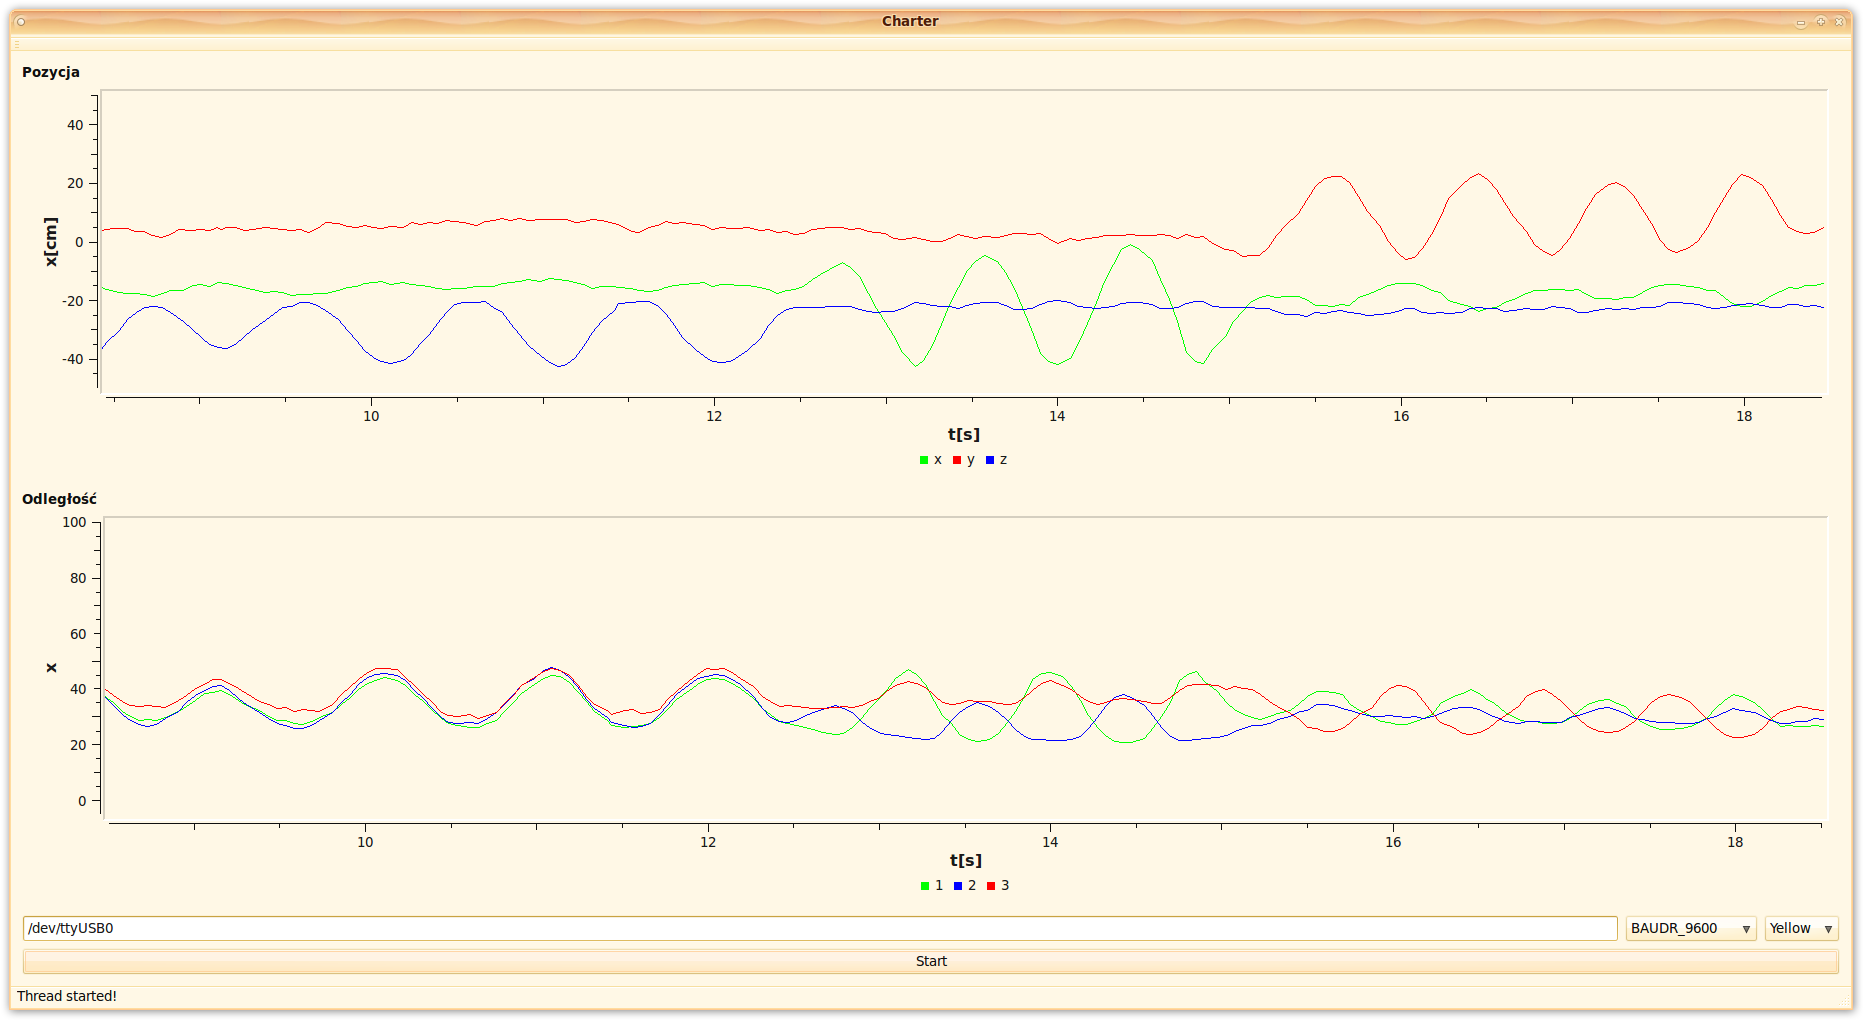
\includegraphics[width=\textwidth]{gfx/charter.png}
  \caption{Program \textsl{Charter} w działaniu}
  \label{fig:charter}
\end{figure}


\subsection{Stickman}
\label{sec:app_stickman}
Trzecią i ostatnią stworzoną aplikacją demo jest \textsl{Stickman}.

Zadaniem tej aplikacji jest odwzorowywanie ruchów użytkownika na ekranie komputera. W głównej części aplikacji rysowana jest figurka imitująca użytkownika, której ruchy rąk odpowiadają ruchom wykonywanym przez użytkownika.

\paragraph{Kalibracja}
Ze względu na możliwość wykorzystania \textsl{Nietoperza} przez różnych użytkowników, do poprawnego działania tej aplikacji wymagane jest przeprowadzenie kalibracji, która dostosowywuje parametry aplikacji do aktualnego użytkownika.

Stworzyłem dwie metody kalibracji:
\begin{itemize}
  \item zwykła,
  \item eksperymentalna.
\end{itemize}
\newline
\newline
\textsl{Kalibracja zwykła} W trybie zwykłym możliwe jest przystosowanie systemu do działania podczas noszenia przez użytkownika. Jest to prostsza z dwóch metod, która wykorzystuje zmiany pozycji względem oczekiwanych osi do odwzorowania ruchów rękoma. Do przeprowadzenia tej kalibracji potrzebne jest pobranie dwóch punktów kontrolnych:
\begin{itemize}
  \item punkt bliski, czyli taki, który znajduje się przy ramieniu użytkownika,
  \item punkt daleki, czyli taki, który znajduje się na w miejscu, w którym będzie ręka użytkownika gdy zostanie ona wyprostowana przed siebie.
\end{itemize}

Na podstawie tych informacji można wyznaczyć długość ręki (długość wektora pomiędzy tymi punktami), przesunięcie ramienia względem początku układu współrzędnych oraz ,,domyślne'' wychylenie ręki w płaszczyznach XZ (poziome) oraz YZ (pionowe).

Każda kolejna pozyskana próbka posłuży do sprawdzenia względnej pozycji wobec punktu bliskiego i dalekiego, a następnie na podstawie odwrotnych równań trygonometrycznych wyznaczone zostaną kąty, o jakie należało będzie obrócić rękę wokół osi X oraz Y.

Rysowana figurka potrafi także, na podstawie długości wektora mającego początek w punkcie bliskim, zaś koniec w aktualnej próbce, zginać rękę. Działanie to jest jednak ograniczone do tylko i wyłącznie jednej płaszczyzny, ponieważ nie przewidziano pozyskania informacji dotyczącej pozycji łokcia. Może zatem istnieć wiele takich ustawień ręki, które spowodują przesunięcie markera do tej samej pozycji, lecz dla aplikacji tej wszystkie one będą jednakowe.
\newline
\newline
\textsl{Kalibracja eksperymentalna} Drugi typ kalibracji, znacznie bardziej złożony od pierwszego, w założeniu pozwalać miał na wykorzystanie \textsl{Nietoperza} z dowolnej pozycji. Pozostało to niestety tylko założeniem, gdyż pomimo mnogich testów i rozważań teoretycznych nie udało się doprowadzić tej metody do stanu pełnej sprawności \ppauza chociaż wielokrotnie wydawało się, że wszystko już działa, to kolejny test pokazywał, że byłem w błędzie.

Do przeprowadzenia tej metody kalibracji wymagany jest jeden punkt więcej niż ma to miejsce przy kalibracji metodą zwykłą. Wynika to z konieczności ponownego ustawienia trójwymiarowego układu współrzędnych, a znając tylko dwa punkty, wiadomo, że są one współliniowe, zaś dookoła prostej możliwy jest dowolny obrót. Trzeci, niewspółliniowy punkt, pozwoli na określenie dokładnej translacji i rotacji.

Odwracając tę transformację, tzn. znajdując takie przekształcenie, które zmieni pozyskany z próbek układ współrzędnych na układ jaki prezentowany jest na rysunku \ref{fig:coordinate_system}, możliwe byłoby dokonywanie normalizacji pozostałych próbek za pomocą tej samej transformacji. Pozwoliłoby to na wykorzystanie metody analogicznej jak w przypadku kalibracji zwykłej.

\paragraph{Struktura programu}
Program oparty został o istniejące wcześniej źródła programu \textsmaller{Charter}. Głównym współdzielonym fragmentem jest klasa \verb|SignalData| oraz kod wątku dokonującego odbierania danych z portu szeregowego (klasa \verb|SamplingThread|). Nie jest to jednak dokładna kopia, gdyż w tym przypadku nie istnieje potrzeba zapewnienia rozszerzalności o nowe markery (człowiek ma tylko dwie ręce, a dodanie śledzenia innych kończyn wymagałoby dopisania ich faktycznej obsługi \ppauza w odróżnieniu od wykresów, gdzie dane dla każdego z markerów są takiej samej struktury). Ponadto program ten nie wykorzystuje biblioteki \textsc{QWT}, wymagane w związku z tym było dostarczenie własnej implementacji pętli zdarzeń.

Wspomniana pętla zdarzeń, stanowiąca ciało wirtualnej metody \verb|run()|, to prosta pętla \verb|while|, która usypiana jest na zadany interwał, po czym wywołuje funkcję odpytującą port o nowe dane. Aby móc poprawnie zakończyć działanie wątku, w każdej iteracji sprawdzany jest stan zmiennej \verb|mRun|, która określa, czy wątek ma wciąż działać \ppauza ma ona wtedy wartość \verb|true|. Podczas zamykania programu usuwany jest obiekt tego wątku, a jego destruktor wywołuje metodę \verb|stop()|, która zapewnia bezpieczny sposób zwolnienia zasobów i pozamykania otwartych połączeń.

Program umożliwia też przeprowadzenie prostego testu wydajności: procedura przekształcania układu współrzędnych wywoływana jest 100000 razy, a sumaryczny czas, jaki zajęło to działanie wypisywany jest na standardowym wyjściu błędów \verb|stderr|.

\section{Protokół}
\label{sec:protocol}
\index{protokół}
Mikrokontroler komunikuje się z komputerem za pomocą standardu \index{RS232}\textsmaller{RS232}, do obsługi którego wykorzystuje moduł \index{USART}\textsmaller{USART}. Aby uzgodnić dane pomiędzy komputerem a mikrokontrolerem, zaprojektowałem protokół, zgodnie z którym następuje przekazanie danych.

Protokół taki powinien zawierać możliwie mało nadmiarowych danych, umożliwiać synchronizację bez względu na moment włączenia nadajnika (mikrokontrolera) względem odbiornika (komputera) oraz zawierać wszystkie potrzebne informacje do odtworzenia położenia wszystkich obsługiwanych markerów.

Mianem \index{raport}\emph{raportu} będziemy nazywać jeden pełen zestaw danych, jakie przesyła do komputera mikrokontroler.

Raport w zaprojektowanym protokole prezentuje rysunek \ref{fig:protocol}.

\begin{figure}
 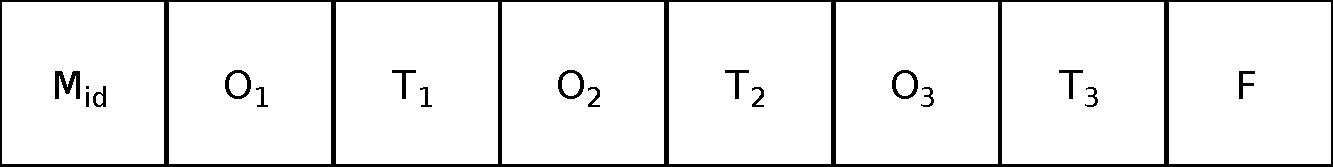
\includegraphics[width=\textwidth]{gfx/diagramy/protokol.pdf}
 \caption[Schemat raportu]{Raport w protokole komunikacji mikrokontrolera z komputerem}
 \label{fig:protocol}
\end{figure}

Każda ramka składa się z ośmiu bajtów, do których należą:
\begin{itemize}
 \item \texttt{M$_\textrm{\texttt{id}}$} \ppauza $id$ markera,
 \item \texttt{O$_n$} \ppauza wartość zmiennej \texttt{ovfCounter} w chwili wygaszenia pinu odbiornika $n$,
 \item \texttt{T$_n$} \ppauza wartość rejestru \texttt{TCNT0} w chwili wygaszenia pinu odbiornika $n$,
 \item \texttt{F} \ppauza zawsze \texttt{0xFF}.
\end{itemize}

Pole \texttt{F} wraz z polem \texttt{M$_\textrm{\texttt{id}}$} służy do synchronizacji danych odbieranych przez komputer. Metodę \index{synchronizacja}synchronizacji prezentuje algorytm \ref{alg:sync}.

\begin{algorithm}
\caption{Metoda synchronizacji danych}
\label{alg:sync}
\begin{algorithmic}[1]
  \REQUIRE \texttt{dane} \ppauza tablica dynamiczna, do której końca dopisywane są przychodzące dane
  \WHILE{\texttt{dane.count() $\geq$ 8}}
    \WHILE{\texttt{dane.count() $\geq$ 8 \&\& (dane[0] != M$_\textrm{\texttt{id}}$ \textbar{}\textbar{} dane[7] != 0x77})}
      \STATE usuń(\texttt{dane[0]})
    \ENDWHILE
  \ENDWHILE
\end{algorithmic}
\end{algorithm}

Należy zauważyć, że poza samymi danym protokołu, pomiędzy kompterem, a mikrokontrolerem przekazywane są również dane kontrolne standardu \index{RS232}RS232:
\begin{itemize}
  \item bity startu,
  \item bity stopu.
\end{itemize}

Zrezygnowałem natomiast z funkcji:
\begin{itemize}
 \item bity parzystości \ppauza te dane kontrolne bardzo słabo spełniają swoją rolę, gdyż są bardzo podatne na zakłócenia, które powodują przestawienie parzystej ilości bitów,
 \item kontrola przepływu \ppauza funkcjonalność nie jest dostępna w mikrokontrolerze.
 \item więcej niż 8 bitów w jednej ramce \ppauza chociaż mikrokontroler oferuje przesłanie do 9 bitów danych w jednej ramce, to wykorzystanie tej funkcjonalności znacznie ograniczyłoby funkcjonalność platformy ze względu na fakt, iż układy stosowane w komputerach rzadko kiedy oferują obsługę takich ramek\graffito{Obsługa 9-bitowych ramek wymaga też specjalnego oprogramowania}, ponadto spowodowałoby dodatkowy narzut pracy na mikrokontrolerze związany z podziałem danych na 9-bitowe części, nie oferując przy tym żadnego wzrostu wydajności \ppauza przesłanie 64 bitów (8 bajtów) wymagałoby i tak 8 ramek.
\end{itemize}

Pełna ramka standardu RS232 składa się zatem z 10 bitów:
\begin{enumerate}
 \item bit startu,
 \item 8 bitów danych,
 \item bit stopu.
\end{enumerate}

Protokół w jego pełnej okazałości demonstruje rysunek \ref{fig:cutecom}.

\begin{figure}
  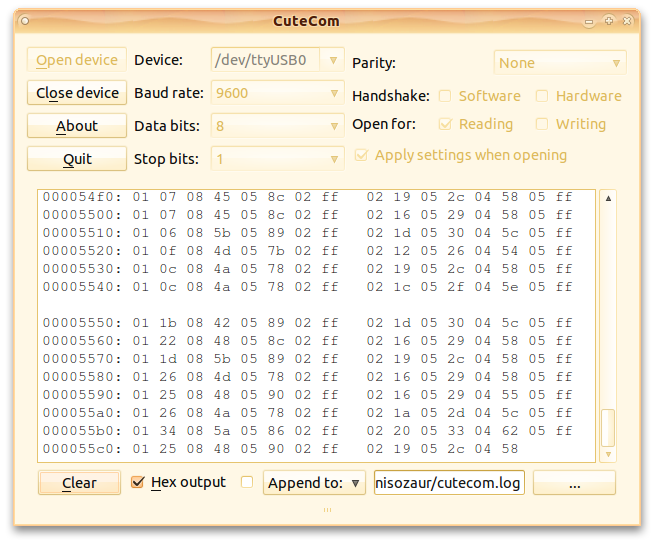
\includegraphics[width=327px]{gfx/cutecom.png}
  \caption{Cutecom \ppauza aplikacja ukazująca ruch na porcie szeregowym wykorzystując opisywany protokół}
  \label{fig:cutecom}
\end{figure}
